\documentclass{article}
\usepackage[utf8]{inputenc}
\usepackage{graphicx}
\usepackage{amsmath}
\usepackage{amsfonts}
\usepackage{amsbsy}
\usepackage{mathrsfs}
\usepackage{appendix}
\usepackage{amsthm}
\usepackage{bbold}
\usepackage{epstopdf}
\usepackage{stmaryrd}
\usepackage[]{algorithm2e}
\usepackage{hyperref}

\usepackage{todonotes}

\title{Reading report for Crossing-Preserving Multi-scale Vesselness}
\author{Leman FENG\\ Email: flm8620@gmail.com\\Website: lemanfeng.com}

\begin{document}
	\maketitle
	\section{Introduction}
	This paper \cite{hannink2014crossing} introduced a new way to detect vessel structures in image. It compares with the previous method \cite{frangi1998multiscale}, and shows that its method can capture crossing of vessels in image, which is hard for \cite{frangi1998multiscale}. This method uses a image transformation called scale-orientation scores to gather features in all direction for each pixel, so that crossing structure can give multiple responses to filters.
	
	I implemented the scale-orientation score transformation in matlab. Result will be given in following sections.
	
	\section{Previous method}
	The previous method this paper compared with is called multi-scale Frangi vesselness filter \cite{frangi1998multiscale}. The idea of Frangi filter is that the Hessian of image can give information about vessel structures. For a 2D image, the eigenvectors and eigenvalues of Hessian at one point describe the pixel values nearby in second order. A elongated shape will have a small eigenvalue corresponding to a eigenvector along the elongated direction, and large eigenvalue in the normal direction. This method can also be used in detecting tube structure in 3D images.
	
	\section{Scale-Orientation score}
	An orientation score of one image is a 3D image $U_f:SE(2)\rightarrow\mathbb{C}$, obtained by convolve input image with a anisotropic wavelet $\psi$ oriented in different directions:
	\begin{equation}
	U_f(\mathbf{x},\theta) = (\bar{\psi_\theta} \star f)(\mathbf{x},\theta)
	\end{equation}
	where $\psi_\theta(\mathbf{x}):=\psi(\mathbf{R}_\theta^{-1} \mathbf{x})$, a rotated version of $\psi$.
	
	The input image can also be reconstructed from its orientation score if the wavelet has good properties. Since this is not used in this paper, I will not talk about it.
	
	\subsection{Interpretation in Fourier domain}
	Convolution of an image with a wavelet is equivalent to multiple their Fourier transformation. Rotating in space domain also corresponds to rotating in frequency domain. The Fourier transform of an anisotropic wavelet is a function preferring certain orientation at frequency domain.
	
	So from my point of view, combining all these above, orientation score can be interpreted as selecting components of an image in its frequency domain with preference at certain orientation. And the region of selection is the support set of wavelet's Fourier transform. This selection region in frequency domain rotates around origin swiping many Fourier components of this image. Each slice of orientation score at angle $\theta$ : $U_f(\cdot,\theta)$ is a selection of Fourier components in image. And if the support of Fourier transform of image is fully covered by the swiping of wavelet's Fourier support, then all components of image are captures, thus the input image can be reconstructed from orientation score.
	
	\subsection{Scale-Orientation score}
	A scale-orientation score is a extension of orientation score. We convolve the input image with the same wavelet, but at multiple scales.
	
	Again, from the point of view in Fourier transform, scaling of wavelets with certain factor corresponds to scaling with the inversed factor in the frequency domain. So the scale-orientation score is actually a swiping at multiple scales in frequency domain.
	
	\subsection{Cake kernels}
	The wavelet chosen by author is called cake kernel \cite{franken2008enhancement}, because in frequency domain the shape of wavelet is like a cut cake : a disk centered at origin is divided in many pieces, each corresponds to a wavelet oriented to one direction. The cake kernel is originally only divided in angle. For multi-scale filter, author divided it further along the radius.
	
	The idea is to divide the disk as a partition of unit, meaning the sum of all wavelets is a indication function of the disk. So author used B-spline function as a basic element for constructing wavelet. We note $B^k$ as the k-th order B-spline function, and polar coordinates in frequency domain is $(\varphi,\rho)$. Let's take $j=0\dots N_\theta-1$ as discretization in angle and $l=0\dots N_\rho-1$ as discretization in radius.
	
	I modified slightly the definition in paper such that it's suitable for implementation.
	
	First we divide long the radius in frequency domain. We choose the minimum and maximum scale as $a_0$ and $a_{N_\rho}$. We want to divide uniformly in log-radius. so the step of discretization $s_\rho=(\log a_{N_\rho} - \log a_0)/N_\rho$. And the support function for radius $\rho$ at scale $l$ is given by
	\begin{equation}
	B_l^k(\rho) = B^k(\frac{\log (\rho a_l
		)}{s_\rho})
	\end{equation}
	with $a_l = a_0 e^{ls_\rho}$.
	Notice that $l=0$ correspond to the smallest wavelet in space domain, while it corresponds to the out most part of the disk in frequency domain. The function $B^k_l$ is plotted in paper, I also give another plot from my matlab implementation in Fig \ref{fig:Bkl}.
	
	\begin{figure}[h]
		\centering
		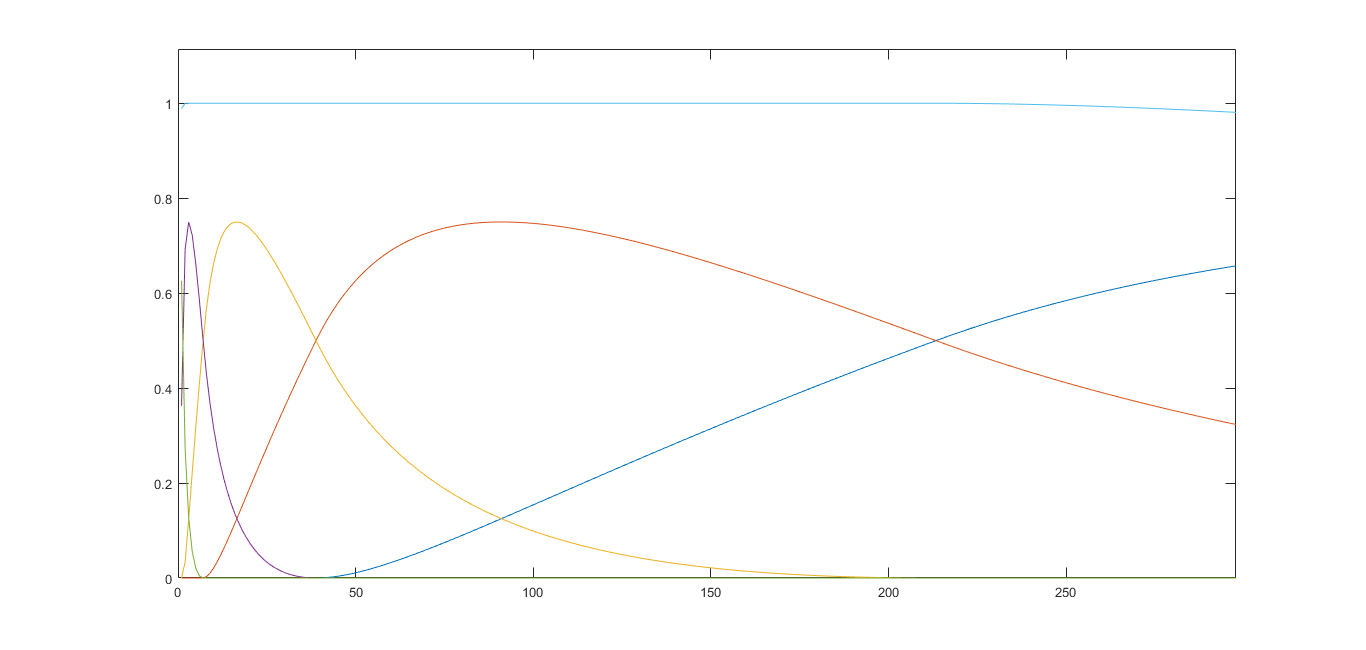
\includegraphics[width=12cm]{scales.png}
		\caption{Partition of unit in radius of frequency domain}
		\label{fig:Bkl}
	\end{figure}
	
	
	Then we divide along angle: 
	\begin{equation}
	A_j(\varphi) = B^k(\frac{(\varphi-j s_\theta)\ \text{mod}\ 2\pi - \pi/2}{s_\theta})
	\end{equation}
	where $s_\theta = 2\pi/N_\theta$ is the step of discretization in angle. And $A_0$ is centered at angle $\pi/2$.
	
	Then we take the product between $A_j$ and $B_l^k$, because taking the Cartesian product of two series of "partition of unit" functions in angle and radius can produce a set of function which is a partition of unit in the disk.
	\begin{equation}
	\boldsymbol{\omega}=(\varphi,\rho) \rightarrow A_j(\varphi) B_l^k(\rho)
	\end{equation}
	Then author multiple this wavelet with a Gaussian function in space domain to keep it local in space
	\begin{equation}
	\tilde{\psi}^{MS}_{jl}(\mathbf{x}) = (\mathcal{F}^{-1}[\boldsymbol{\omega}\rightarrow A_j(\varphi) B_l^k(\rho)])(\mathbf{x})G_{s_x,s_y}(\mathbf{x})
	\end{equation}
	the gaussian product modifies the wavelets and they no longer forms a partition of unit on disk. So another normalization step is needed:
	\begin{equation}
	\psi^{MS}_{jl}(\mathbf{x}) = (\mathcal{F}^{-1}[M^{-1}\mathcal{F}[\tilde{\psi}^{MS}_{jl}](\boldsymbol{\omega})])(\mathbf{x})
	\end{equation}
	where $M(\boldsymbol{\omega}) = N_\rho^{-1} N_\theta^{-1} \sum_{l}\sum_{j} |\mathcal{F}[\tilde{\psi}^{MS}_{jl}](\boldsymbol{\omega})|$
	
	Some example of final wavelets $\psi^{MS}_{jl}$ is shown in Fig \ref{fig:wavelet}
	\begin{figure}[h]
		\centering
		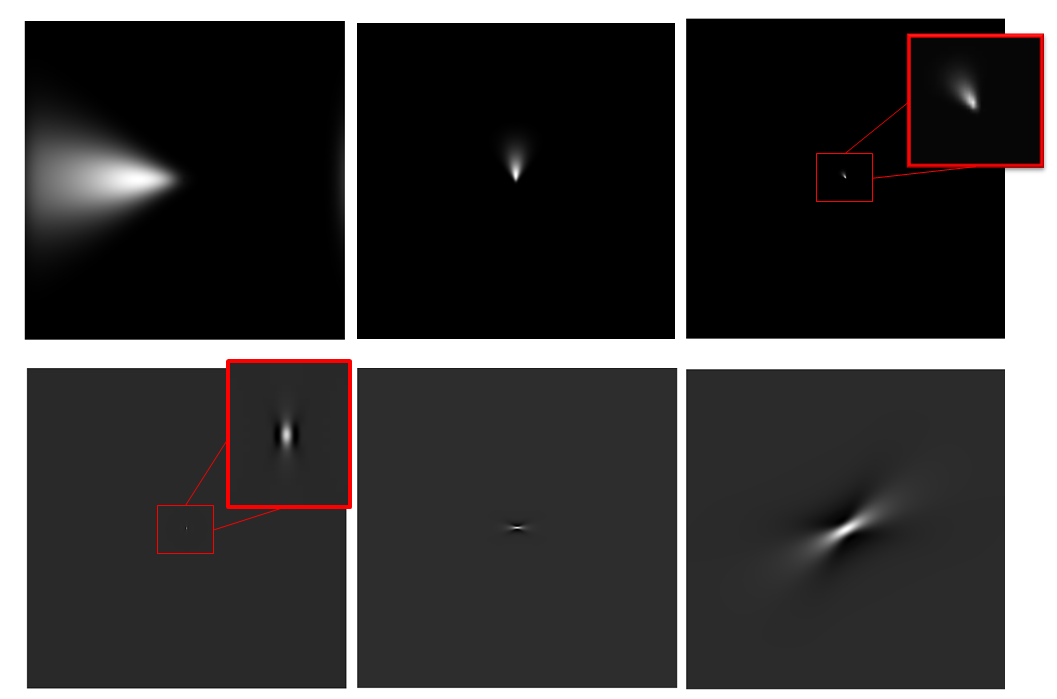
\includegraphics[width=12cm]{wavelets.png}
		\caption{Three wavelets in space (up) and frequency (bottom) domain.}
		\label{fig:wavelet}
	\end{figure}

	Once the wavelets is ready, scale-orientation score can be simply constructed by multipling the Fourier transform of image by the Fourier of all wavelets, giving a 4D image at last.

	\section{Vesselness filtering}
	The vesselness filtering part is basically the same as Frangi's method \cite{frangi1998multiscale}. For each point in the 3D orientation score at one scale, we evaluate the Hessian. To avoid the problem of aliasing when we derive image, we take a convolution with a Gaussian kernel on image. This is equivalent to convolve the image with the derivative of Gaussian kernel.
	
	But taking the convolution and derivation in group $SE(2)$ is not trivial. We need to make sure that our operator is left-invariant for the lie group $SE(2)$. This left-invarience property requires the derivation direction must rotate together with the angle $\theta$, and the convolution kernel is twisted along $\theta$. 
	
	Since this part is a natural extension of previous method, and left-invariant operator is not trivial to implement, I didn't implement this part in my matlab code.
	
	
	\section{Implementation detail}
	I implemented the cake kernel in matlab. The code is available online at \href{https://github.com/flm8620/Crossing-Preserving-Multi-scale-Vesselness}{my github}. All operations involving Fourier transform can be implemented by Discret Fourier transform. The different is a scaling constant, which can be ignored because the inverse transform will cancel it out.
	
	I took a image of size 1025*1025. I select 5 scales from $a_0=0.002$ to $a_4=10$. And 12 orientations are taken. I use order-2 B-spline function with support in interval $[-1.5, 1.5]$. So there are in total 5*12 = 60 wavelets.
	
	I create one test image as shown in Fig \ref{fig:score}. Three slices of scale-orientation score are also shown. This three slice correspond the convolution result with three wavelets in Fig \ref{fig:wavelet}.
	
	\begin{figure}[h]
		\centering
		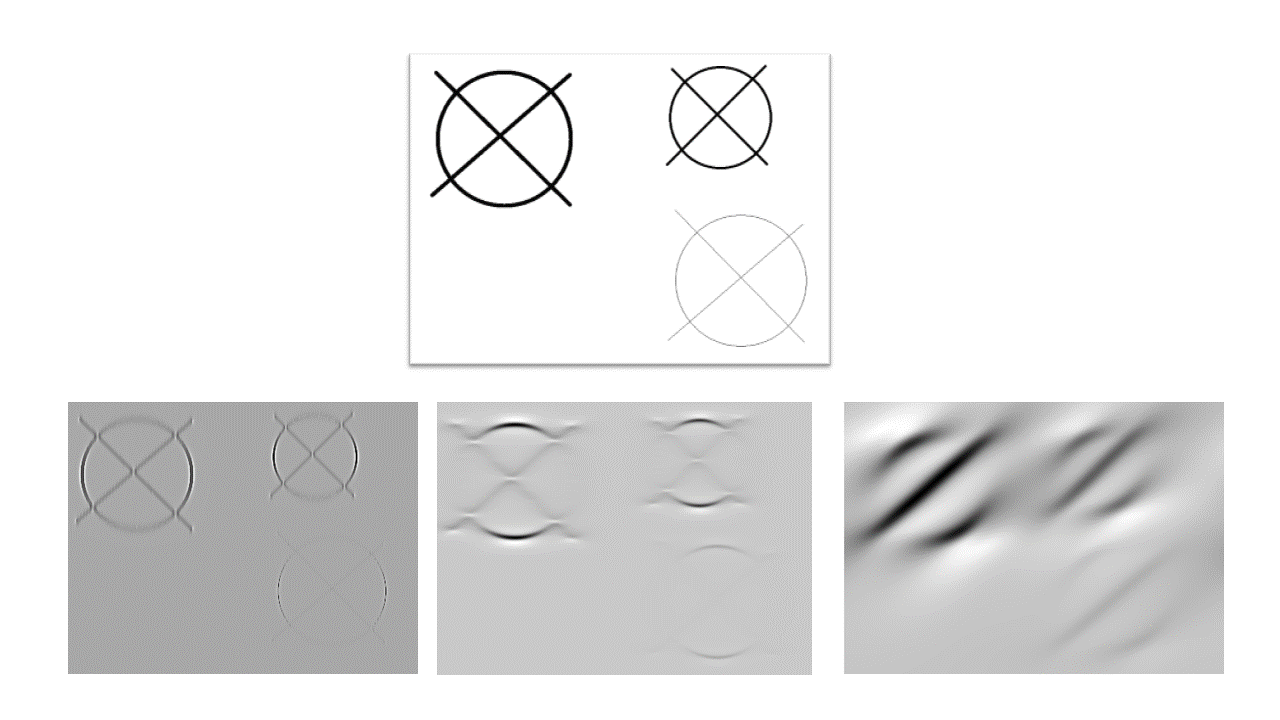
\includegraphics[width=12cm]{scores.png}
		\caption{Three slice of scale-orientation scale of one test image, corresponding to three wavelet in Fig \ref{fig:wavelet}}
		\label{fig:score}
	\end{figure}
	We can see from Fig \ref{fig:score} that the response of score is specific to particular orientation and scale.
\bibliographystyle{unsrt}
\bibliography{sample}
\end{document}
